% RECOMMENDED %%%%%%%%%%%%%%%%%%%%%%%%%%%%%%%%%%%%%%%%%%%%%%%%%%%
\documentclass[graybox]{svmult}

% choose options for [] as required from the list
% in the Reference Guide

\usepackage{type1cm} % activate if the above 3 fonts are not available on your system
\usepackage{makeidx} % allows index generation
\usepackage{graphicx} % standard LaTeX graphics tool when including figure files
\usepackage{multicol} % used for the two-column index
\usepackage[bottom]{footmisc} % places footnotes at page bottom
\usepackage{svg}
\usepackage{booktabs}
\usepackage{newtxtext}
\usepackage{newtxmath} % selects Times Roman as basic font
\usepackage{lipsum}
\usepackage{comment}

\usepackage[style=apa, backend=biber]{biblatex}

\DeclareFieldFormat{apacase}{#1}

\DeclareLanguageMapping{american}{american-apa}
\let \citeNP \cite
\let \citeA \textcite
\let \cite \parencite

\bibliography{./references.bib}

% see the list of further useful packages
% in the Reference Guide

\makeindex             % used for the subject index
                       % please use the style svind.ist with
                       % your makeindex program

%%%%%%%%%%%%%%%%%%%%%%%%%%%%%%%%%%%%%%%%%%%%%%%%%%%%%%%%%%%%%%%%%%%%%%%%%%%%%%%%%%%%%%%%%

\begin{document}
\title*{Enhancing Quality of Virtual Meetings through Facial and Vocal Emotion Recognition}

\titlerunning{Enhancing Quality of Virtual Meetings through Facial and Vocal Emotion Recognition}
% Use \titlerunning{Short Title} for an abbreviated version of
% your contribution title if the original one is too long
\author{Page, Philipp\inst{a}$_{1}$ \and
Karaus, Kilian\inst{a}$_{2}$ \and
Donner, Maximilian\inst{a}$_{3}$}
\authorrunning{Page, Karaus, Donner}

\institute{
 University of Cologne, Albertus-Magnus-Platz, 50923 Cologne, Germany
}

\maketitle
\abstract{Due to the COVID-19 pandemic, presentations via video conferencing software are part of the daily routine for many people. However, the quality of the presentations, which are used in universities to transfer knowledge but also in widespread areas of the business world, differs significantly. In order to improve meeting quality we have developed a web application allowing presenters to gather real-time metrics about the people's mood during the meeting. In particular, the proposed system tracks the emotional state of the meeting participants and combines this data with subjective ratings. Emotional data of the audience is collected with the help of face recognition. At the same time, the systems analyzes the speaker's voice to deduce transmitted emotions. The collected data can help researchers to form hypotheses about what makes a ``good'' meeting. Additionally, presenters are able to change their presentation style during a meeting or in future meetings after performing a post hoc analysis.}

\footnotetext[1]{Corresponding author: Philipp Page, e-mail: mail@philipp-page.de}
\footnotetext[2]{Corresponding author: Kilian Karaus, e-mail: kkaraus@smail.uni-koeln.de}
\footnotetext[3]{Corresponding author: Maximilian Donner, e-mail: mdonner@smail.uni-koeln.de}
\addtocounter{footnote}{3}

\section{Introduction}
\label{sec:intro}
The global pandemic caused by the Covid-19 virus had a strong impact on the professional environment in 2020 and in the first half of 2021. Employers sent their staff into the home office as far as possible. A survey found that before the Corona crisis, around 40 percent of employees in companies worked from home in the home office. During the pandemic, this share increased by about 20 percentage points to around 60 percent. This has sometimes meant that normal business meetings, whether with clients or colleagues, have had to take place via video conferencing platforms such as ZOOM or similar. Nevertheless, in the business world, as well as in university life, presentations are an essential part of sharing knowledge. It is important to present in the right way to have the best possible impact on the audience. For a good presentation, the way in which the presenters express their information using emotions is therefore of essential importance \cite{derrico_tracking_2019}.

Emotions in presentations can be transmitted in various ways, such as vocabulary and emotional words like “grateful”, “unique”, and “honored” when expressing inspiration, whether the presenter communicates enthusiastically vs. indifferently or the provided gestures and facial expressions while presenting, such as smiling, being surprised or sad etc \cite{zeng_emoco_2019, rosler_reducing_2021}. Using deep neural networks, in particular Convolutional Neural Networks (CNNs), it is possible to determine emotions from facial expressions with a high degree of accuracy. Many researchers have shown, for example, that their deep learning-based methods perform very well on various datasets for recognizing emotions in the face \cite{ko_brief_2018}. Voice emotions regarding voice can also be determined using such neural networks. Using facial emotion recognition, some researchers analyzed the relationship between facial expressions and the learning process to monitor and measure student engagement \cite{de_carolis_engaged_2019}, for example, to provide personalized feedback to improve the learning experience. 

In our seminar paper, we look more closely at the relationship between emotion through facial expressions and through voice in presentation. The goal of this seminar is to build a web app (\url{www.moody.digital}) that measures and stores both facial and vocal emotions in real-time during live presentations with the help of CNNs and trained emotion recognition models. In addition, feedback from the participants is requested after each presentation in order to put the presentations into context. Such an evaluation could help researchers and practitioners to better understand the inherent relationship between emotions and presentations, and furthermore to improve the quality of presentations in the long term, thereby promoting better knowledge transfer. Therefore, our research question is as follows:
\vspace{3mm}
\newline
\emph{(RQ)\quad How can we design a system to collect real-time feedback with the goal to reduce video conference fatigue?}

\section{Related Work}
\label{sec:related_work}
In the following sections, a literature review is conducted. The first two parts describe the current scientific approaches to measure emotions for both faces and voices using deep neural networks. The third part explains the relationship between the quality of presentations and emotions.

\subsection{Facial Emotion Recognition}
\label{subsec:related_work_facial_emotion_recognition}
Facial Emotion Recognition (FER) is a subarea of computer vision and deals with the prediction of human emotional states using facial mimics and expressions in images, moving pictures or videos \cite{jain_extended_2019}.
According to \citeA{rosler_reducing_2021} FER literature and research suggest firstly, two separate ways of feature generation: manually or automatically through a deep neural network. Secondly, they outline the differentiation of their underlying emotional model, which is either based on discrete emotional states or on continuous dimensions \cite{rosler_reducing_2021}. Five fundamental discrete emotional states, for example identified by \citeA{ekman_universal_1997}, are happiness, sadness, fear / surprise, disgust and anger. There is several different literature recognizing other fundamental emotional states, and thus a set definition is not available. Also, the continuous dimensions are defined divergently. Given an instance, \citeA{mollahosseini_affectnet_2017} use two or three dimensions to explain emotions, with valence or pleasantness as one dimension and arousal or activation as the other.

In this work we will focus on leveraging discrete emotional states, since it is more maturely researched and more suitable to generate features using deep learning based approaches. Considering the amount of developments of recent years in deep learning, we concentrate on using the available variety of deep neural networks as the most appropriate technique in FER \cite{jain_extended_2019}. We could also focus on FER approaches that use handcrafted features and which are according to \citeA{ko_brief_2018} often deployed in the following three steps. First, face and facial component detection from the input image. Second, spatial and temporal feature extraction. And third, expression classification by e.g. Support Vector Machine or Random Forests to recognize emotional states. Although this manual way often leads to accurate results and requires less computational resources, many researches, such as \citeA{jung_joint_2015}, showed the superiority of deep learning algorithms with for example CNNs over handcrafted approaches.

One of the main advantages of CNNs and other neural networks is the possibility to automatically learn features from the input images, which is called ``end-to-end'' learning \cite{ko_brief_2018}. This Moody Prototype also uses a CNN implementation via the \texttt{face-api.js} library, which is described further in Section~\ref{subsec:method_facial_emotion_recognition}. These in the context of facial emotion recognition most used CNNs operate and process images, as the name discloses, ``convolutionally'' and can take spatial information into consideration \cite{ko_brief_2018, rosler_reducing_2021}. Thus, we utilize a CNN to recognize the emotional states of \citeA{ekman_universal_1997}: happy, sad, fearful, angry, surprised and disgusted. Additionally, since audiences listen and their faces appear often simply neutrally, we added another emotional state to our recognition model, called ``neutral''.

\section{Hypothesis}
\label{sec:hypothesis}

\section{Method}
\label{sec:method}

\subsection{System Architecture}
\label{subsec:method_system_architecture}

\subsection{Facial Emotion Recognition}
\label{subsec:method_facial_emotion_recognition}

\subsection{Vocal Emotion Recognition}
\label{subsec:method_vocal_emotion_recognition}

\subsubsection{Data Preprocessing}
\label{subsubsec:method_vocal_emotion_recognition_data_preprocessing}

\subsubsection{AlexNet Architecture}
\label{subsubsec:method_vocal_emotion_recognition_alexnet_architecture}
\section{Results}
\label{sec:results}
\section{Discussion}
\label{sec:Discussion}
\section{Limitations and Future Work}
\label{sec:limitations_and_future_work}
\input{./sections/07_summary.tex}
\newpage
\section*{Appendix: Relational Data Model}
\label{app:appendix_relational_data_model}
\begin{figure}[ht]
\label{fig:erd}
\centering
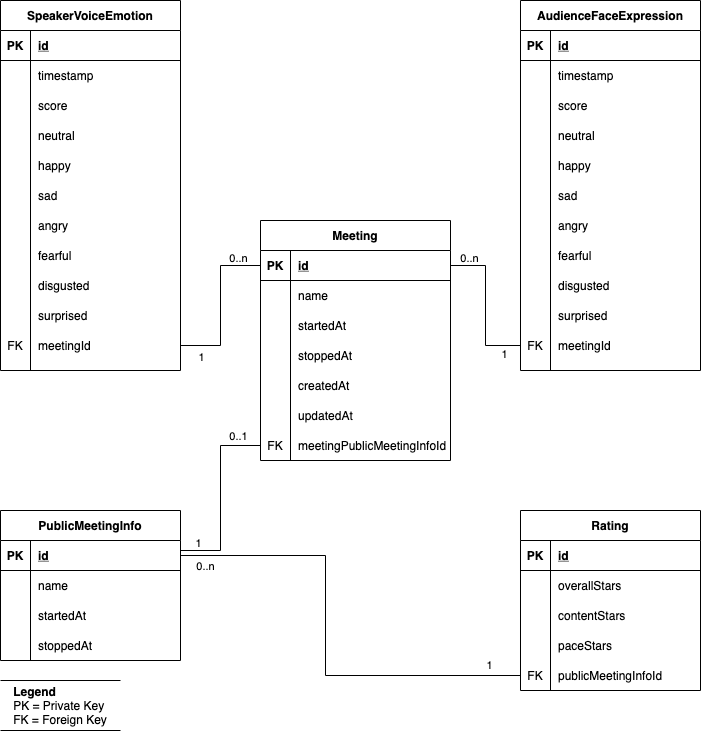
\includegraphics[width=1\textwidth]{assets/erd.png}
\caption{The entity relationship diagram (ERD) for the database structure of Moody. Relationships are modeled in UML style. Each table has an additional owner field  storing the user id from AWS Cognito which is omitted in the illustration for brevity.}
\end{figure}

\newpage
\printbibliography
\end{document}
